%%%%%%%%%%%%%%%%%%%%%%%%%%%%%%%%%%%%%%%%%%%%%%%%%%%%%%%%%%%%%%%%%%%%%%%%%%%%%%%
% EDC Gravity Sector (BLOCK-003): A 5D-First Derivation Program
% From bulk+brane+GHY+Israel to an effective 4D Newton coupling
%
% Status: OPEN / Research Program (not results)
%%%%%%%%%%%%%%%%%%%%%%%%%%%%%%%%%%%%%%%%%%%%%%%%%%%%%%%%%%%%%%%%%%%%%%%%%%%%%%%
\documentclass[11pt,a4paper]{article}

\usepackage[utf8]{inputenc}
\usepackage[T1]{fontenc}
\usepackage{amsmath,amssymb,amsthm}
\usepackage{geometry}
\geometry{margin=2.5cm}
\usepackage{hyperref}
\hypersetup{colorlinks=true, linkcolor=blue!60!black, citecolor=blue!60!black, urlcolor=blue!60!black}
\usepackage{booktabs}
\usepackage{longtable}
\usepackage{enumitem}
\usepackage{tikz}
\usetikzlibrary{arrows.meta, shapes.geometric, positioning, calc}
\usepackage{tcolorbox}
\tcbuselibrary{skins,breakable}

% Epistemic tag macros (consistent with EDC repo style)
\newcommand{\tagBL}{\textcolor{blue!70!black}{[BL]}}
\newcommand{\tagI}{\textcolor{green!50!black}{[I]}}
\newcommand{\tagP}{\textcolor{orange!80!black}{[P]}}
\newcommand{\tagOPEN}{\textcolor{red!70!black}{[OPEN]}}
\newcommand{\tagDer}{\textcolor{purple!70!black}{[Der]}}

% Box environments
\newtcolorbox{statusbox}{
  colback=yellow!5!white,
  colframe=yellow!50!black,
  fonttitle=\bfseries,
  title=Epistemic Status,
  breakable
}

\newtcolorbox{programbox}{
  colback=blue!5!white,
  colframe=blue!50!black,
  fonttitle=\bfseries,
  breakable
}

\newtcolorbox{warningbox}{
  colback=red!5!white,
  colframe=red!50!black,
  fonttitle=\bfseries,
  title=Warning: Anti-Circularity,
  breakable
}

\title{\textbf{EDC Gravity Sector (BLOCK-003):}\\[0.3em]
A 5D-First Derivation Program\\[0.5em]
\large From Bulk+Brane+GHY+Israel to an Effective 4D Newton Coupling}
\author{EDC Research Program\\[0.3em]
\small\textit{Status: \tagOPEN{} --- Derivation roadmap, not results}}
\date{2026-02-02\\[0.3em]\small\textit{Program note / roadmap; not a results paper}}

\begin{document}

\maketitle

%===============================================================================
\begin{abstract}
%===============================================================================
BLOCK-003 designates the open problem of deriving the 4D Newton coupling $G_N$ within the Elastic Diffusive Cosmology (EDC) framework without circular input.
This note provides a structured derivation program: starting from the 5D bulk Einstein--Hilbert action with Gibbons--Hawking--York boundary terms and brane tension, through Israel junction conditions, to extraction of an effective 4D gravitational coupling.
A central requirement is \emph{anti-circularity}: inputs used here (bulk parameters $\kappa_5$, $\Lambda_5$, $\sigma$) must be independent of those already employed in EM/nuclear sector closures.
An explicit Input Ledger separates allowed from prohibited inputs.
No numerical closure is claimed; no fit to $G_N^{\mathrm{obs}}$ is performed.
Closure would require deriving the correct scaling $G_N \sim \kappa_5^2 / R_\xi$ (or equivalent) and recovering the 4D Newtonian limit at large distances.
This note is a standalone companion to the EDC nuclear pinning monograph, which remains gravity-out-of-scope.
\end{abstract}

%===============================================================================
\section{Epistemic Status \& Scope}
\label{sec:epistemic}
%===============================================================================

\begin{statusbox}
\textbf{Status: \tagOPEN{}/\tagP{}.}
This paper is a \emph{derivation roadmap}, not a completed result.
The gravity sector (BLOCK-003) remains open.
No numerical predictions for $G_N$ or gravitational signatures are made here.
\end{statusbox}

\paragraph{What this paper is.}
A structured research program for deriving 4D gravity from a 5D brane-world setup consistent with EDC conventions.
The derivation chain is outlined; key steps are identified; acceptance criteria are defined.

\paragraph{What this paper is not.}
\begin{itemize}[nosep]
    \item Not a claim that gravity is ``solved'' in EDC.
    \item Not a source of new physics claims or predictions.
    \item Not a replacement for the nuclear pinning monograph (which remains gravity-out-of-scope).
\end{itemize}

\paragraph{Epistemic tags used.}
\begin{itemize}[nosep]
    \item \tagBL{}: Standard brane-world formalism (textbook results).
    \item \tagI{}: Identification or interpretation within EDC framework.
    \item \tagP{}: EDC-specific postulate (not independently derived).
    \item \tagOPEN{}: Open problem; derivation not complete.
\end{itemize}

\paragraph{Notation summary.}
\begin{center}
\small
\begin{tabular}{ll}
\toprule
\textbf{Symbol} & \textbf{Meaning} \\
\midrule
$X^A = (w, x^i, \xi)$ & Bulk coordinates ($A = 0,\ldots,4$) \\
$w$ & Bulk time \\
$t$ & Brane operational time; $w = v_{\mathrm{scan}} t$ \\
$\Sigma^4$ & 4D brane hypersurface \\
$\sigma$ & Brane tension \\
$\kappa_5^2 = 8\pi G_5$ & 5D gravitational coupling \\
$\Lambda_5$ & Bulk cosmological constant \\
$h_{\mu\nu}$, $K_{\mu\nu}$ & Induced metric, extrinsic curvature \\
\bottomrule
\end{tabular}
\end{center}

%===============================================================================
\section{Canonical 5D Geometric Setup (EDC-Consistent)}
\label{sec:geometry}
%===============================================================================

\paragraph{Bulk coordinates \tagBL{}/\tagI{}.}
EDC postulates a 5D Lorentzian bulk manifold $\mathcal{M}^5$ with coordinates
\begin{equation}
    X^A = (w, x^1, x^2, x^3, \xi), \qquad A = 0, \ldots, 4,
\end{equation}
where $w$ is the bulk time coordinate and $\xi$ is the extra spatial coordinate.

\paragraph{Brane and operational time \tagI{}.}
A 4D brane $\Sigma^4$ is embedded in $\mathcal{M}^5$.
Brane observers measure operational time $t$, related to bulk time via the scan map $w = v_{\mathrm{scan}} t$.
In many applications one sets $v_{\mathrm{scan}} = 1$; the conceptual distinction is retained.

\paragraph{Induced metric \tagBL{}.}
The brane inherits an induced metric from the bulk:
\begin{equation}
    h_{\mu\nu}(x) = \partial_\mu X^A \, \partial_\nu X^B \, g_{AB}(X)\big|_{\Sigma}, \qquad \mu, \nu = 0, \ldots, 3.
\end{equation}

\paragraph{Metric ansatz (optional) \tagP{}.}
A specific warped metric (e.g., $ds^2_5 = e^{-2A(\xi)} \eta_{\mu\nu} dx^\mu dx^\nu + d\xi^2$) may be adopted for concrete calculations.
Such an ansatz is \emph{not} prescribed here as ``the'' EDC metric; any choice must be labeled \tagP{} and justified separately.

%===============================================================================
\section{Action Principle (5D-First)}
\label{sec:action}
%===============================================================================

The total action consists of three parts \tagBL{} (see \cite{MTW,Wald} for standard GR formulation):

\begin{programbox}
\textbf{5D Action Components}

\textbf{1. Bulk Einstein--Hilbert + cosmological term:}
\begin{equation}
    S_{\mathrm{bulk}} = \frac{1}{2\kappa_5^2} \int_{\mathcal{M}^5} d^5X \sqrt{-g^{(5)}} \left( R^{(5)} - 2\Lambda_5 \right)
    \label{eq:S_bulk}
\end{equation}

\textbf{2. Gibbons--Hawking--York boundary term:}
\begin{equation}
    S_{\mathrm{GHY}} = \frac{1}{\kappa_5^2} \int_{\Sigma^4} d^4x \sqrt{-h} \, K
    \label{eq:S_GHY}
\end{equation}

\textbf{3. Brane action (tension + matter):}
\begin{equation}
    S_{\mathrm{brane}} = \int_{\Sigma^4} d^4x \sqrt{-h} \left( -\sigma + \mathcal{L}_{\mathrm{matter}} \right)
    \label{eq:S_brane}
\end{equation}
\end{programbox}

\paragraph{Notation.}
\begin{itemize}[nosep]
    \item $\kappa_5^2 = 8\pi G_5$ is the 5D gravitational coupling.
    \item $\Lambda_5$ is the bulk cosmological constant.
    \item $K = h^{\mu\nu} K_{\mu\nu}$ is the trace of the extrinsic curvature.
    \item $\sigma$ is the brane tension.
\end{itemize}

\paragraph{Why GHY is required \tagBL{}.}
The GHY term \cite{York1972,GH1977} is necessary for a well-posed variational principle when the manifold has boundaries.
Without it, the variation of $R^{(5)}$ produces boundary terms that do not vanish, making the action principle ill-defined.

%===============================================================================
\section{Junction Conditions \& Field Equations}
\label{sec:junction}
%===============================================================================

\paragraph{Derivation chain (outline) \tagBL{}.}

\begin{center}
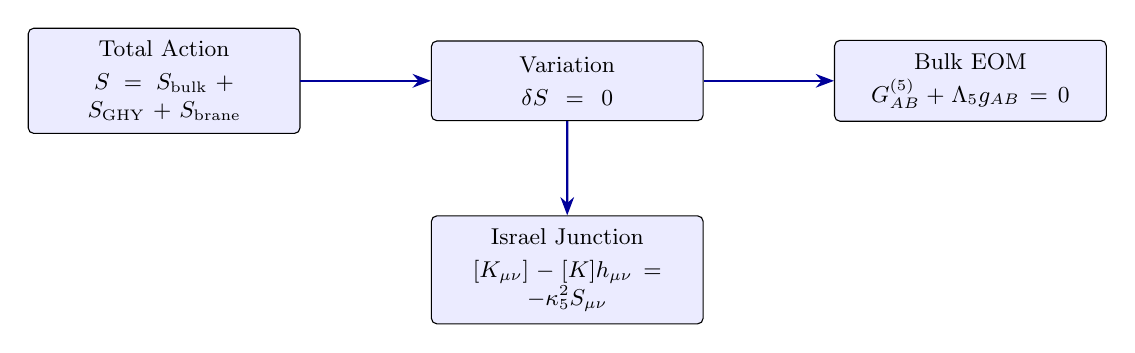
\begin{tikzpicture}[>=Stealth, node distance=1.8cm, scale=0.92, transform shape,
    box/.style={rectangle, draw, fill=blue!8, text width=3.4cm, text centered,
                minimum height=1.1cm, font=\small, rounded corners=2pt,
                inner sep=5pt}]

    \node[box] (action) {Total Action\\[2pt]$S = S_{\mathrm{bulk}} + S_{\mathrm{GHY}} + S_{\mathrm{brane}}$};
    \node[box, right=of action] (vary) {Variation\\[2pt]$\delta S = 0$};
    \node[box, right=of vary] (eom) {Bulk EOM\\[2pt]$G_{AB}^{(5)} + \Lambda_5 g_{AB} = 0$};
    \node[box, below=1.3cm of vary] (israel) {Israel Junction\\[2pt]$[K_{\mu\nu}] - [K] h_{\mu\nu} = -\kappa_5^2 S_{\mu\nu}$};

    \draw[->, thick, blue!60!black] (action) -- (vary);
    \draw[->, thick, blue!60!black] (vary) -- (eom);
    \draw[->, thick, blue!60!black] (vary) -- (israel);
\end{tikzpicture}
\end{center}

\paragraph{Israel junction conditions \tagBL{}.}
At the brane location, the discontinuity in extrinsic curvature is related to the brane stress-energy \cite{Israel1966}:
\begin{equation}
    [K_{\mu\nu}] - [K] h_{\mu\nu} = -\kappa_5^2 \left( T_{\mu\nu}^{\mathrm{brane}} - \frac{1}{3} T h_{\mu\nu} \right)
    \label{eq:israel}
\end{equation}
For a tension-dominated brane ($T_{\mu\nu} = -\sigma h_{\mu\nu}$), this becomes:
\begin{equation}
    [K_{\mu\nu}] = -\frac{\kappa_5^2}{3} \sigma \, h_{\mu\nu} + \kappa_5^2 \left( \tau_{\mu\nu} - \frac{1}{3} \tau h_{\mu\nu} \right)
\end{equation}
where $\tau_{\mu\nu}$ is the matter stress-energy on the brane (excluding tension).

\paragraph{Status.}
Equations~\eqref{eq:israel} are standard results \tagBL{}.
Their application to a specific EDC metric ansatz requires further work \tagOPEN{}.

%===============================================================================
\section{Linearized Gravity \& Effective 4D Newton Coupling (Program)}
\label{sec:linearized}
%===============================================================================

\begin{statusbox}
\textbf{Status: \tagOPEN{}.}
This section outlines the \emph{required steps} to extract $G_N$.
No calculation is performed here.
\end{statusbox}

\paragraph{Goal.}
Obtain an effective 4D gravitational potential on $\Sigma^4$ with $1/r$ long-distance behavior and identify $G_N$ in terms of 5D parameters.

\paragraph{Required steps.}

\begin{enumerate}[label=\textbf{Step \arabic*:}, leftmargin=2.5cm]
    \item \textbf{Choose background.} Select a specific 5D metric ansatz (flat, warped, or EDC-specific) and solve for the background geometry.

    \item \textbf{Linearize.} Expand $g_{AB} = g_{AB}^{(0)} + h_{AB}$ and derive linearized field equations.

    \item \textbf{Mode decomposition.} Perform Kaluza--Klein decomposition; identify tensor modes (4D graviton), scalar modes (radion/brane-bending), and their mass spectra.

    \item \textbf{Normalization.} Normalize mode functions with respect to the appropriate inner product to obtain canonical kinetic terms.

    \item \textbf{Brane-to-brane propagator.} Compute the Green function for metric perturbations sourced and observed on the brane.

    \item \textbf{Extract $G_N$.} From the long-distance ($r \gg$ compactification scale) limit of the brane-to-brane potential, identify the coefficient as $G_N$.
\end{enumerate}

\paragraph{Expected form (schematic) \tagOPEN{}.}
In typical brane-world scenarios \cite{RS1999,Maartens2010}, the effective Newton constant takes the form:
\begin{equation}
    G_N \sim \frac{\kappa_5^2}{R_\xi} \quad \text{or} \quad G_N \sim \kappa_5^2 \cdot (\text{warp factor integral})
    \label{eq:GN_schematic}
\end{equation}
The precise form depends on the metric ansatz and must be derived, not assumed.

%===============================================================================
\section{Input Ledger (Anti-Circularity)}
\label{sec:ledger}
%===============================================================================

\begin{warningbox}
To avoid circular reasoning, we must distinguish:
\begin{itemize}[nosep]
    \item \textbf{Allowed inputs:} Parameters that can be used to derive $G_N$ without circularity.
    \item \textbf{Prohibited inputs:} Parameters already used to close the EM/nuclear sectors (e.g., $\alpha$, $r_e$).
\end{itemize}
Using prohibited inputs to derive $G_N$ would make gravity a consistency check, not a prediction.
\end{warningbox}

\begin{center}
\renewcommand{\arraystretch}{1.3}
\begin{longtable}{p{2.5cm}p{2cm}p{7cm}}
\toprule
\textbf{Quantity} & \textbf{Status} & \textbf{Source / Notes} \\
\midrule
\endfirsthead
\toprule
\textbf{Quantity} & \textbf{Status} & \textbf{Source / Notes} \\
\midrule
\endhead
\bottomrule
\endfoot

$\kappa_5$ or $M_5$ & \tagOPEN{} & 5D Planck mass; must be independently fixed or predicted. \\

$\Lambda_5$ & \tagP{} & Bulk cosmological constant; may be set by consistency (e.g., flat brane requirement). \\

$R_\xi$ & \tagP{}/\tagOPEN{} & Compactification scale; geometry parameter. If derived from $\sigma$, see below. \\

$\sigma$ (intrinsic) & \tagP{} & Brane tension as bulk property. \textbf{Allowed:} if derived from $\sigma = 2\pi R_\xi^2 \rho_P$ (pressure integration). \\

$\sigma_{\mathrm{eff}}$ & \tagI{} & Effective tension at EM scale. \textbf{Prohibited:} if extracted from $\alpha$, $r_e$ (circularity risk). \\

$\alpha$ & \tagBL{} & Fine structure constant. \textbf{Prohibited} for gravity derivation (used in EM closure). \\

$r_e$ & \tagBL{} & Classical electron radius. \textbf{Prohibited} for gravity derivation (used in EM closure). \\

$m_e$ & \tagBL{} & Electron mass. \textbf{Prohibited} for gravity derivation (used in EM closure). \\

Warp factor $A(\xi)$ & \tagP{}/\tagOPEN{} & If used, must be derived or postulated independently. \\

\end{longtable}
\end{center}

\paragraph{Guiding principle.}
For $G_N$ to qualify as a \emph{prediction} of EDC (not merely a consistency check), it must be derivable from:
\begin{itemize}[nosep]
    \item Geometric parameters ($R_\xi$, warp profile) determined by 5D dynamics, OR
    \item The intrinsic tension $\sigma$ derived from bulk pressure integration (non-circular path).
\end{itemize}

%===============================================================================
\section{Pipeline Schematic}
\label{sec:pipeline}
%===============================================================================

\begin{figure}[ht]
\centering
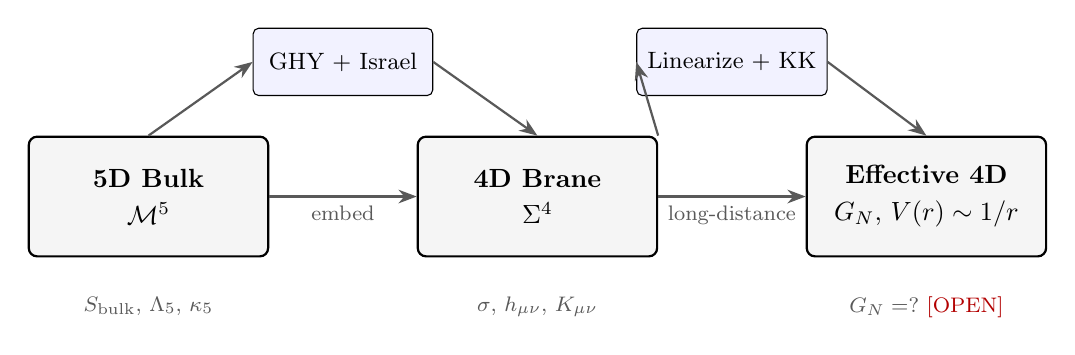
\begin{tikzpicture}[>=Stealth, scale=0.95, transform shape,
    bigbox/.style={rectangle, draw, thick, fill=gray!8, minimum width=3.2cm,
                   minimum height=1.6cm, align=center, rounded corners=3pt,
                   inner sep=8pt},
    smallbox/.style={rectangle, draw, fill=blue!5, minimum width=2.4cm,
                     minimum height=0.9cm, text centered, font=\small,
                     rounded corners=2pt, inner sep=4pt},
    arrow/.style={->, thick, gray!70!black}]

    % Main boxes - evenly spaced
    \node[bigbox] (bulk) at (0,0) {\textbf{5D Bulk}\\[2pt]$\mathcal{M}^5$};
    \node[bigbox] (brane) at (5.2,0) {\textbf{4D Brane}\\[2pt]$\Sigma^4$};
    \node[bigbox] (eff) at (10.4,0) {\textbf{Effective 4D}\\[2pt]$G_N$, $V(r) \sim 1/r$};

    % Process boxes - centered above arrows
    \node[smallbox] (ghy) at (2.6,1.8) {GHY + Israel};
    \node[smallbox] (lin) at (7.8,1.8) {Linearize + KK};

    % Main horizontal arrows
    \draw[arrow] (bulk) -- (brane) node[midway, below, font=\footnotesize] {embed};
    \draw[arrow] (brane) -- (eff) node[midway, below, font=\footnotesize] {long-distance};

    % Process arrows
    \draw[arrow] (bulk.north) -- (ghy.west);
    \draw[arrow] (ghy.east) -- (brane.north);
    \draw[arrow] (brane.north east) -- (lin.west);
    \draw[arrow] (lin.east) -- (eff.north);

    % Labels below boxes
    \node[below=0.4cm of bulk, font=\footnotesize, text=gray!70!black] {$S_{\mathrm{bulk}}$, $\Lambda_5$, $\kappa_5$};
    \node[below=0.4cm of brane, font=\footnotesize, text=gray!70!black] {$\sigma$, $h_{\mu\nu}$, $K_{\mu\nu}$};
    \node[below=0.4cm of eff, font=\footnotesize, text=gray!70!black] {$G_N = ?$ \tagOPEN{}};

\end{tikzpicture}
\caption{Schematic derivation pipeline for BLOCK-003 (program overview). Starting from the 5D bulk action, apply GHY and Israel junction conditions at the brane, linearize, and extract the effective 4D Newton coupling $G_N$. Status: \tagOPEN{}.}
\label{fig:pipeline}
\end{figure}

%===============================================================================
\section{Connection to Nuclear Pinning Monograph}
\label{sec:connection}
%===============================================================================

This paper is a \emph{standalone companion} to the EDC nuclear pinning monograph (``Topological Pinning Model for Nuclear Structure and Superheavy $\alpha$-Decay Predictions'').

\paragraph{Separation of concerns.}
\begin{itemize}[nosep]
    \item The nuclear monograph addresses nuclear binding, $\alpha$-decay, and topological pinning. Gravity is explicitly out-of-scope there (BLOCK-003).
    \item This paper addresses the gravity derivation program. Nuclear physics is not treated here.
\end{itemize}

\paragraph{No modifications to the monograph.}
This paper does not add, remove, or modify any content in the nuclear monograph.
The monograph may contain a single-sentence pointer: ``See separate gravity program note for BLOCK-003.''
No other cross-references are required.

%===============================================================================
\section{Roadmap \& Acceptance Criteria}
\label{sec:roadmap}
%===============================================================================

The following acceptance criteria define what is needed to close BLOCK-003:

\begin{center}
\renewcommand{\arraystretch}{1.3}
\begin{longtable}{p{1.5cm}p{9cm}p{2cm}}
\toprule
\textbf{ID} & \textbf{Criterion} & \textbf{Status} \\
\midrule
\endfirsthead
\toprule
\textbf{ID} & \textbf{Criterion} & \textbf{Status} \\
\midrule
\endhead
\bottomrule
\endfoot

AC-G1 & Well-posed 5D action with bulk, GHY, and brane terms explicitly written. & \tagBL{} Done \\

AC-G2 & Israel junction conditions derived or correctly quoted with proper index structure. & \tagBL{} Done \\

AC-G3 & Specific metric ansatz chosen and background solution obtained. & \tagOPEN{} \\

AC-G4 & Linearized perturbation equations derived around background. & \tagOPEN{} \\

AC-G5 & KK modes identified, classified (tensor/scalar), and normalized. & \tagOPEN{} \\

AC-G6 & Brane-to-brane propagator computed; long-distance limit shows $1/r$ behavior. & \tagOPEN{} \\

AC-G7 & $G_N$ extracted and expressed in terms of 5D parameters without circularity. & \tagOPEN{} \\

AC-G8 & Consistency check: $G_N$ value compatible with measured Newton constant (order of magnitude or better). & \tagOPEN{} \\

AC-G9 & Parameter counting: clearly state what is input vs.\ what is predicted. & \tagOPEN{} \\

AC-G10 & Reproducibility: derivation steps documented such that an independent researcher can verify. & \tagOPEN{} \\

\end{longtable}
\end{center}

\paragraph{Current status.}
Only AC-G1 and AC-G2 are addressed in this document (as standard results).
All other criteria remain \tagOPEN{}.

%===============================================================================
\section{Conclusion}
\label{sec:conclusion}
%===============================================================================

This document outlines a structured 5D-first research program for BLOCK-003 (gravity sector) within EDC.
The main elements are:
\begin{enumerate}[nosep]
    \item A derivation roadmap from 5D action to effective 4D $G_N$.
    \item An explicit \emph{input ledger} to prevent circular reasoning.
    \item Defined acceptance criteria (AC-G1 through AC-G10) for closure.
\end{enumerate}

No physics results or numerical predictions are claimed.
This note is intended as a starting point for future work on the EDC gravity sector.

%===============================================================================
% References
%===============================================================================

\begin{thebibliography}{9}

\bibitem{MTW}
C.~W. Misner, K.~S. Thorne, and J.~A. Wheeler,
\textit{Gravitation} (W.~H. Freeman, San Francisco, 1973).

\bibitem{Wald}
R.~M. Wald,
\textit{General Relativity} (University of Chicago Press, 1984).

\bibitem{York1972}
J.~W. York,
``Role of conformal three-geometry in the dynamics of gravitation,''
\textit{Phys.\ Rev.\ Lett.}\ \textbf{28}, 1082 (1972).

\bibitem{GH1977}
G.~W. Gibbons and S.~W. Hawking,
``Action integrals and partition functions in quantum gravity,''
\textit{Phys.\ Rev.\ D}\ \textbf{15}, 2752 (1977).

\bibitem{Israel1966}
W.~Israel,
``Singular hypersurfaces and thin shells in general relativity,''
\textit{Nuovo Cimento B}\ \textbf{44}, 1 (1966).

\bibitem{RS1999}
L.~Randall and R.~Sundrum,
``Large mass hierarchy from a small extra dimension,''
\textit{Phys.\ Rev.\ Lett.}\ \textbf{83}, 3370 (1999).

\bibitem{Maartens2010}
R.~Maartens and K.~Koyama,
``Brane-world gravity,''
\textit{Living Rev.\ Relativ.}\ \textbf{13}, 5 (2010).

\end{thebibliography}

\end{document}
